% \documentclass[12pt,handout,xcolor=pdftex,dvipsnames,table]{beamer} %For handouts.
\documentclass{beamer}
%\usepackage{pgfpages} %For handouts.
% This is the file main.tex
% \usepackage{handoutWithNotes}
\usepackage{subcaption} % subfigure
\usepackage{hyperref}
\usepackage{graphicx}
\usepackage[en-US]{datetime2} % fix warning of \author[*]{\today}
\usepackage{lmodern}% http://ctan.org/pkg/lm (For special Fonts)
\usepackage{ragged2e} % justify document
\usepackage{tikz}
\usepackage{smartdiagram}
\usepackage{xcolor}
% \usepackage{subfig}
\usepackage{multicol}

\mode<presentation>
\setbeamertemplate{blocks}[rounded][shadow=true]
\usetheme{Dresden} % so so
\setbeamertemplate{page number in head/foot}[totalframenumber]
\setbeamertemplate{navigation symbols}{} %take out the navigation symbols
\setbeamertemplate{caption}[numbered] %enumerate the caption and tables
\usefonttheme[stillsansseriflarge]{structureitalicserif}
  
%\mode<handout>{\setbeamercolor{background canvas}{bg=black!5}} %For handouts.
% \pgfpagesuselayout{4 on 1 with notes}[a4paper,border shrink=5mm]
  
%\makeatletter %reset the numbering on the subfigures (1)
%\@addtoreset{subfigure}{figure} %reset the numbering on the subfigures (2)
%\makeatother %reset the numbering on the subfigures (3)

%For Large figures
%\includegraphics[width=\linewidth,height=\textheight,keepaspectratio]{SMS}

\title{Kubernetes Vagrant CI / CD} % (optional, only for long titles)
\subtitle{
	\href{https://github.com/thanos1983/kubernetesVagrant}
    		{GitHub Project Repo: kubernetesVagrant}
}
\author[Athanasios Garyfalos]{Sample of Work of fully automate build, deploy, validate containers locally. Deploy on a k8s cluster and validations.} % (optional, for multiple authors)
% {A.~Garyfalos \and A.~Garyfalos2 \and A.~Garyfalos3}
\institute[garyfalos@cpan.org] % (optional)
{
	\\
	\medskip
	{
	% \emph{A.atga12@student.bth.se}
	% \emph{Another Author email}
	% \emph{Another Author}
	}
}
\vspace*{-0.5cm}
% \date{Date: \today} % Multi page content
% \subject{Sample of Work Demonstration Django Rest Framework}

% \AtBeginSection[]{
%  \begin{frame}
%    \frametitle{Table of Contents}
%    \tableofcontents[currentsection]
%  \end{frame}
% }

\AtBeginSubsection[]{
  \begin{frame}<beamer>
    \begin{multicols}{2}
      \tableofcontents[currentsection,hideothersubsections]
    \end{multicols}
  \end{frame}
}

\begin{document}
	\begin{frame}[noframenumbering]
  \begin{center}
    % Upper part of the page
    
\includegraphics[width=.8\textwidth]{png/kubernetesLogo}\\ % [0.3cm]
  \end{center}
  \titlepage
\end{frame}

	% \section*{Copyright Disclaimer}
  \begin{frame}
    \begin{justify}
      {\justifying Copyright \alert{Disclaimer}: This program is free software: you can redistribute it and/or modify it under the terms of the GNU General Public License as published by the Free Software Foundation, either version 3 of the License, or (at your option) any later version.
      \bigbreak
      This program is distributed in the hope that it will be useful, but WITHOUT ANY WARRANTY; without even the implied warranty of MERCHANTABILITY or FITNESS FOR A PARTICULAR PURPOSE.  See the GNU General Public License for more details.
      \bigbreak
      You should have received a copy of the GNU General Public License along with this program.  If not, see.~\cite{gnuLicences} }
    \end{justify}
\end{frame}

	\section*{Contents}
\begin{frame}[allowframebreaks]
\setbeamercovered{dynamic}%Makes the text appear before it presents nice!!!! 
	\frametitle{Outline}
	\tableofcontents[pausesections, sections={1-4}]
		\framebreak
	\tableofcontents[pausesections, sections={5-8}]
\end{frame}
	\section{Introduction} \label{sec:k8sFuntamentals}
\subsection{Kubernetes Elements}

\begin{frame}{High level description}
\setbeamercovered{dynamic}%Makes the text appear before it presents nice!!!!
	\begin{columns}[T] % contents are top vertically aligned
		\begin{column}{5cm} % each column can also be its own environment
			\begin{itemize}
				\item<+-| alert@+> VM Vs Container.
				\item<+-| alert@+> What is a Pod (pea pod)?
				\item<+-| alert@+> Container Runtime Interface(s) (CRI).
					\begin{itemize}
						\item<+-| alert@+> Docker
						\item<+-| alert@+> Podman
						\item<+-| alert@+> CRI-O
					\end{itemize}
				\item<+-| alert@+> Docker Vs Podman.
				\item<+-| alert@+> What is actually k8s?
			\end{itemize}
		\end{column}
		\begin{column}{5cm} % alternative top-align that's better for graphics
		\begin{figure}
			\only<1>{%
				\centering Virtual Machine Vs Container
				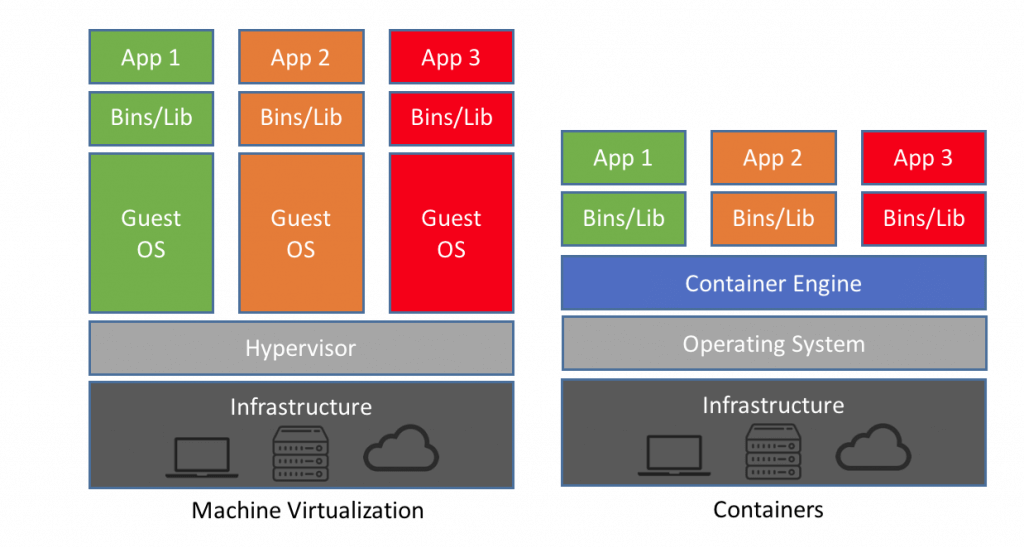
\includegraphics[width=\columnwidth, height=0.5\textheight]{./png/container}
			}%
			\only<2>{%
				\centering Container inside Pod
				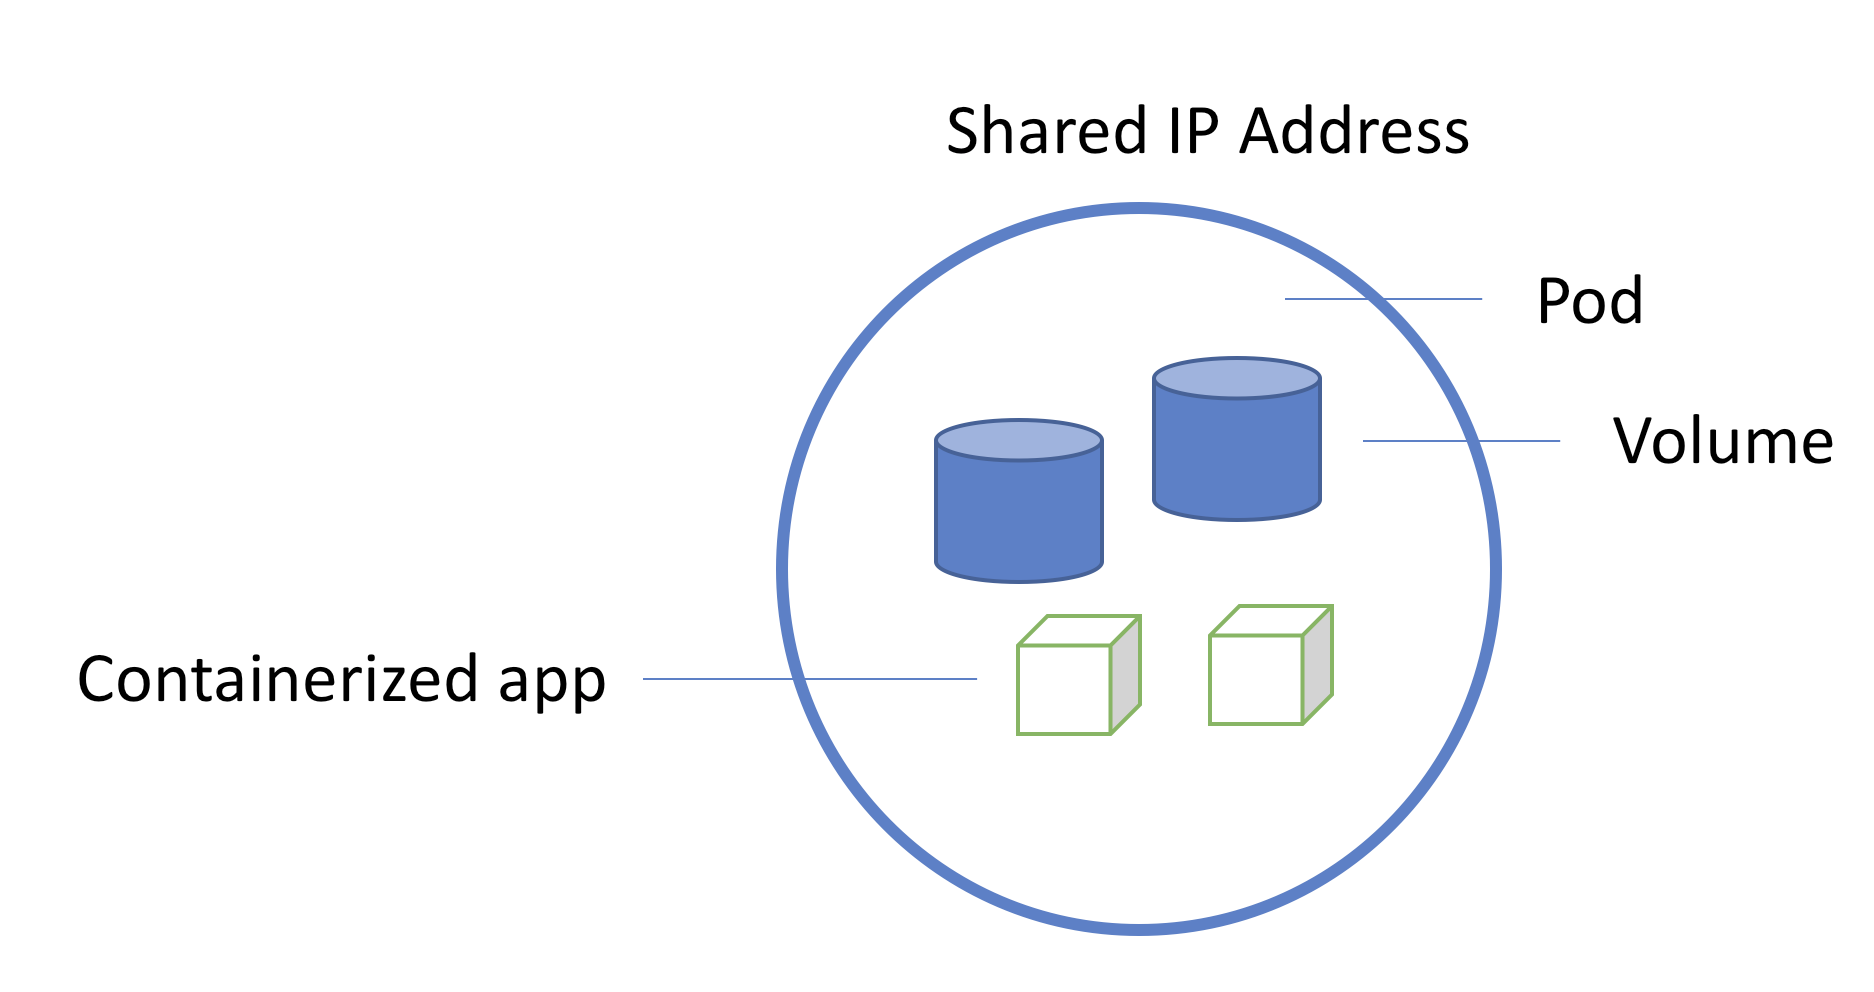
\includegraphics[width=\columnwidth, height=0.5\textheight]{./png/pod}
			}%
			\only<3>{%
				\centering Container Runtime Interface
				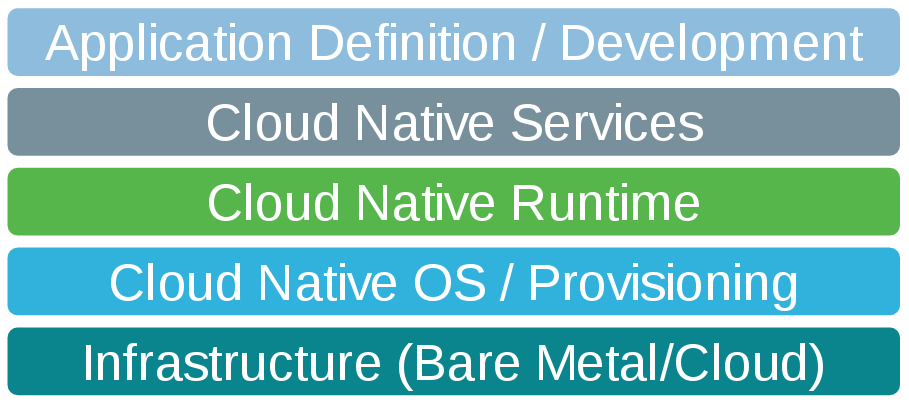
\includegraphics[width=\columnwidth, height=0.5\textheight]{./png/cri}
			}%
			\only<4>{%
				\centering Most known (insecure) socket
				
\includegraphics[width=\columnwidth, height=0.5\textheight]{./png/docker}
			}%
			\only<5>{%
				\centering Most unknown (secure) socket
				
\includegraphics[width=\columnwidth, height=0.5\textheight]{./png/buildah-podman}
			}%
			\only<6>{%
				\centering Lightest fastest socket
				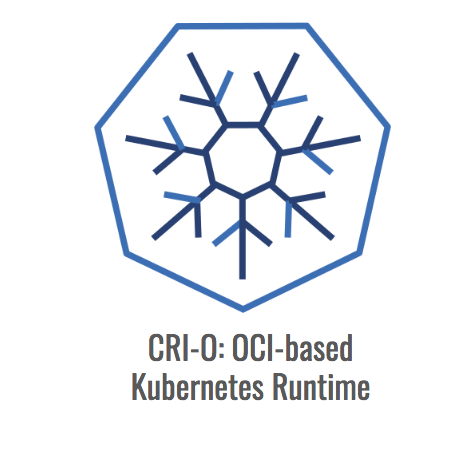
\includegraphics[width=\columnwidth, height=0.5\textheight]{./png/crio}
			}%
			\only<7>{%
				\centering Read about it
				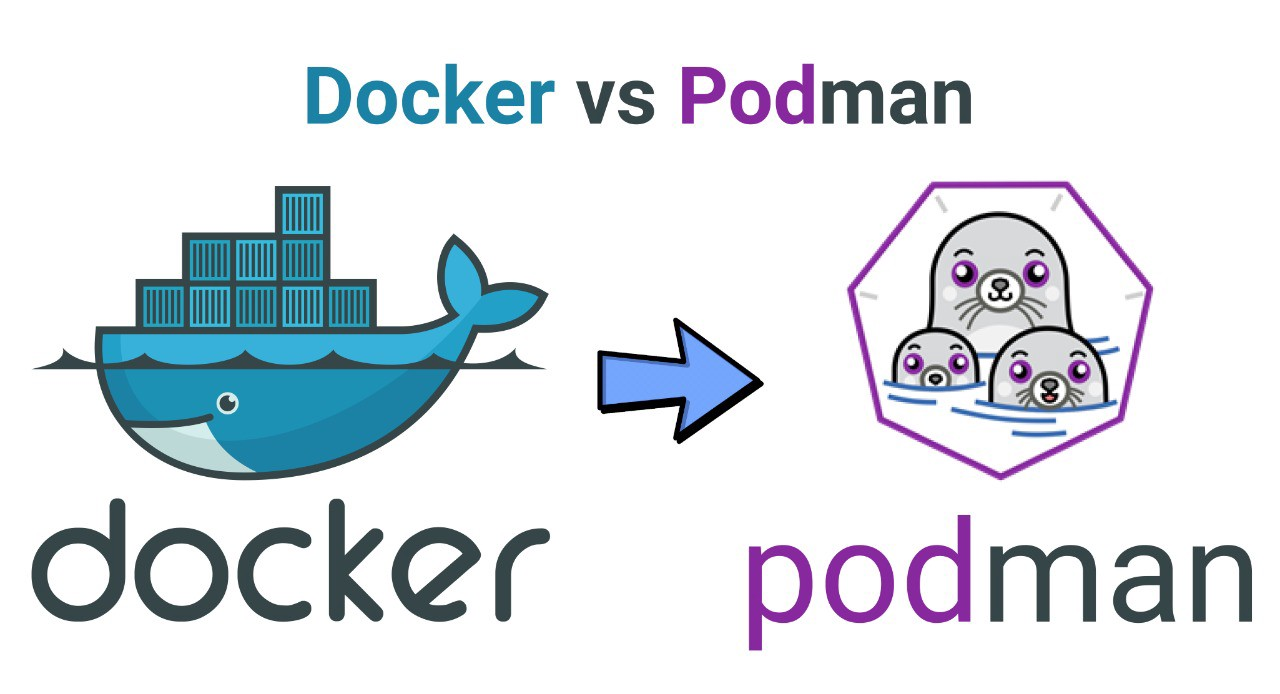
\includegraphics[width=\columnwidth, height=0.5\textheight]{./png/dockervspodman}
			}%
			\only<8>{%
				\centering Is a puzzle of elements
				
\includegraphics[width=\columnwidth, height=0.5\textheight]{./png/k8sPuzzle.jpg}
			}%
			\caption{k8s Overview} \label{fig:largeFigure}
		\end{figure}
		\end{column}
	\end{columns}
\end{frame}

	\section{Wireless Platform}
\label{sec:wireless}
  \subsection{Key Factors and Components}

\begin{frame}{Hardware Description}
\setbeamercovered{dynamic}%Makes the text appear before it presents nice!!!!
    \begin{columns}[t] % contents are top vertically aligned
      \begin{column}[T]{5cm} % each column can also be its own environment
        \begin{itemize}
            \item<+-| alert@+> Single component of the base winding Figure:%~\autoref{fig:structure}.
            \item<+-| alert@+> Receiver platform values Figure:~1b.
            \item<+-| alert@+> Worst coupling position Figure:~1c.
            \item<+-| alert@+> Best coupling position Figure:~1d.
          \end{itemize}  
      \end{column}
    \begin{column}[T]{5cm} % alternative top-align that's better for graphics
      \begin{figure}
        \only<1>{%
        %\vspace*{-1.5cm}
          \subfloat[First subfigure\label{fig:a}]{
            \includegraphics[height=2cm,width=3cm]{./png/structure}
          }
          \label{fig:1}
        }
        \only<2>{%
        %\vspace*{-1.5cm}
          \subfloat[Second subfigure\label{fig:b}]{
            \includegraphics[height=2cm,width=3cm]{./png/receiver}
          }
          \label{fig:2}
        }
        \only<3>{%
        %\vspace*{-1.5cm}
          \subfloat[Third subfigure\label{fig:c}]{
            \includegraphics[height=2cm,width=3cm]{./png/worst}
          }
          \label{fig:3}
        }
        \only<4>{%
        %\vspace*{-1.5cm}
          \subfloat[Fourth subfigure\label{fig:d}]{
            \includegraphics[height=2cm,width=3cm]{./png/best}
          }
          \label{fig:4}
        }
        \captionsetup{justification=centering} %Center a two line caption
        \caption{Project Positioning Analysis} \protect\label{fig:5}%~\cite{wsn}
      \end{figure}
    \end{column}
  \end{columns}
\end{frame}

%\subsection{Best and Worst Performance Based on Positioning}

%\begin{frame}{Theory Vs Practical Experimentation}
%\setbeamercovered{dynamic}%Makes the text appear before it presents nice!!!! 
%    \begin{columns}[t] % contents are top vertically aligned
%      \begin{column}[T]{5cm} % each column can also be its own environment
%        \begin{itemize}
%            \item<+-| alert@+> Best Position Simulation (\ding{108})
%            \item<+-| alert@+> Worst Position Simulation (\alert{\ding{110}})
%            \item<+-| alert@+> Best Position Measured (\ding{108})
%            \item<+-| alert@+> Worst Position Measured (\alert{\ding{110}})
%            \item<+-| alert@+> Simulation is a perfect line, in ``\alert{Theory}''
%            \item<+-| alert@+> Practical measuring shows ``\alert{150KHz}''!
%        \end{itemize}
%      \end{column}
%    \begin{column}[T]{5cm} % alternative top-align that's better for graphics
%      \begin{figure}
%        \vspace*{-10pt}
%        \centerline{\includegraphics[scale=0.7]{./png/efficiency}}
%        \vspace*{10pt}
%        \captionsetup{justification=centering} %Center a two line caption
%        \caption{Simulation Vs Real Time Efficiency~\cite{wsn}}
        %\includegraphics[options]{path_to_image}syntax
%      \end{figure}
%    \end{column}
%  \end{columns}
%\end{frame}

	\section{Implementation}
\label{sec:implementation}
  \subsection{Neural Network Algorithm Implementation}
  
\begin{frame}
  \centering
  \begin{figure}
    \only<1-3>{
        \begin{subfigure}[b]{0.3\textwidth}
          \caption{Free Positioning}
                \includegraphics[width=\textwidth,height=\textwidth]{./png/multiple}
                \label{fig:guided}
                \setcounter{subfigure}{0}% Reset subfigure counter
        \end{subfigure}\hfill
        }
    \only<2-3>{
        ~ %add desired spacing between images, e. g. ~, \quad, \qquad etc.
          %(or a blank line to force the subfigure onto a new line)
        \begin{subfigure}[b]{0.3\textwidth}
        \setcounter{subfigure}{1}% Reset subfigure counter
          \caption{Neural Network}
                \includegraphics[width=\textwidth,height=\textwidth]{./png/neural}
                \label{fig:free}
        \setcounter{subfigure}{0}% Reset subfigure counter
        \end{subfigure}\hfill
        }
    \only<3-3>{
        ~ %add desired spacing between images, e. g. ~, \quad, \qquad etc.
          %(or a blank line to force the subfigure onto a new line)
        \begin{subfigure}[b]{0.3\textwidth}
            \setcounter{subfigure}{2}% Reset subfigure counter
          \caption{Matlab Output}
                \includegraphics[width=\textwidth,height=\textwidth]{./png/output}
                \label{fig:multiple}
        \end{subfigure}%
        }
        \caption{Different wireless charging approaches~\label{fig:animals}~\cite{wsn}}
  \end{figure}
  \begin{itemize}[<+->]
      \item<1-| alert@1>> Free positioning charging based on Inductive coupling~\cite{wireless}.
      \item<2-| alert@2>> Based on RLoad and Frequency Input and Output ~\cite{wireless}. %\ref{fig:free}
      \item<3-| alert@3>> Simulation of Matlab Output based on RLoad as an Input~\cite{wireless}. %\ref{fig:multiple}
    \end{itemize} 
\end{frame}
	\section{Architecture} \label{sec:architecture}
\subsection{Minimal Kubernetes Components}

\begin{frame}{Kubernetes Minimal Core Components}
\setbeamercovered{dynamic}%Makes the text appear before it presents nice!!!!
	\begin{columns}[T] % contents are top vertically aligned
		\begin{column}{5cm} % each column can also be its own environment
			\resizebox{5cm}{!}{%
					\smartdiagramset{set color list={orange!60,
											green!50!lime!60,
											magenta!60
											},
											uniform connection color=true
					}
					\smartdiagram[constellation diagram]{k8s,
												Socket(s),
												Main\\Packages,
												Network\\Elements
					}
			}%
		\end{column}
		\begin{column}{5cm} % alternative top-align that's better for graphics
			\begin{itemize}
				\item<+-| alert@+> Socket:
				\begin{itemize}
						\item<+-| alert@+> Containerd (Docker)
						\item<+-| alert@+> CRI-O
					\end{itemize}
				\item<+-| alert@+> Main Packages:
				\begin{itemize}
					\item<+-| alert@+> kubeadm
					\item<+-| alert@+> kubelet
					\item<+-| alert@+> kubectl
				\end{itemize}
				\item<+-| alert@+> Network Elements
					\begin{itemize}
						\item<+-| alert@+> Calico~\cite{gnuLicences}
						\item<+-| alert@+> WeaveNet~\cite{gnuLicences}
						\item<+-| alert@+> Cilium~\cite{gnuLicences}
					\end{itemize}
			\end{itemize}
		\end{column}
	\end{columns}
\end{frame}

\subsection{My view of Kubernetes Minimal Core Components}

\begin{frame}{Local Auto Deployment}
\setbeamercovered{dynamic}%Makes the text appear before it presents nice!!!!
	\begin{columns}[T] % contents are top vertically aligned
		\begin{column}{5cm} % alternative top-align that's better for graphics
			\begin{itemize}
				\item<+-| alert@+> Previous Elements
				\item<+-| alert@+> Ingress Controller:
					\begin{itemize}
						\item<+-| alert@+> NGINX~\cite{kubernetesNetworking}
						\item<+-| alert@+> HaProxy~\cite{kubernetesNetworking}
					\end{itemize}
				\item<+-| alert@+> Metrics (HPA)
				\item<+-| alert@+> Dashboard
					\begin{itemize}
						\item<+-| alert@+> Self Signed CA
					\end{itemize}
				\item<+-| alert@+> Serveless Functions, Functions as a Service (FaaS)
				\item<+-| alert@+> Operatin System:
					\begin{itemize}
						\item<+-| alert@+> Ubuntu
					\end{itemize}
			\end{itemize}
		\end{column}
		\begin{column}{5cm} % each column can also be its own environment
			\resizebox{5cm}{!}{%
					\smartdiagram[constellation diagram]{k8s,
												Socket(s),
												Main\\Packages,
												Network\\Elements,
												Ingress\\Controller,
												Dashboard,
												Metrics,
												Serverless\\Functions
					}
			}%
		\end{column}
	\end{columns}
\end{frame}
	\section{Demo}
\subsection{Demo CI / CD}

\begin{frame}
\setbeamercovered{dynamic}
	\begin{center}
		\Huge \textcolor{cyan}{\emph{Coming up: Demo}}
	\end{center}
\end{frame}
	\section{Summary}
  \subsection{Key points repetition}

\begin{frame}
\setbeamercovered{dynamic}
  \begin{exampleblock}{Summary}
    \begin{itemize}[<+->]
      \item In section~``\nameref{sec:group}'' page ``\ref{sec:group}'' we mentioned member positions and responsibilities. 
      \item In section~``\nameref{sec:wireless}'' page ``\ref{sec:wireless}'' we mentioned hardware components and best/worst positions.
      \item In section~``\nameref{sec:implementation}'' page ``\ref{sec:implementation}'' we mentioned our approach and proposed solution to the problem \pause
    \end{itemize}
  \end{exampleblock}
  \begin{exampleblock}{Extra Notes}
    \begin{itemize}[<+->]
      \item Both the Conference paper and the Presentation where written in \alert{\LaTeX}
      \item Due to the quality of the output it exceeds our expectations!~\cite{research}
    \end{itemize}
  \end{exampleblock}
\end{frame}

\subsection*{Questions}
\begin{frame}
%\begin{overlayarea}{\textwidth}{3cm}
    %\only<1>{Some text for the first slide.\\Possibly several lines long.}
    %\only<2>{Replacement on the second slide.}
%\end{overlayarea}
  \begin{itemize}
     \Large
    \item \colorbox{yellow}{Thanks a lot – questions \& comments?}
  \end{itemize} 
\end{frame}

	\section{Bibliography}
\subsection*{Web and Articles}

\begin{frame}[allowframebreaks]
	\frametitle<presentation>{References}
	\bibliographystyle{amsalpha}
		\begin{thebibliography}{10}
		%\setbeamertemplate{bibliography item}[online]
		\setbeamertemplate{bibliography item}{
\includegraphics[width=1.5em]{./png/gnu}}
			\bibitem{gnuLicences}
				GNU LESSER GENERAL PUBLIC LICENSE
				\newblock {\emph{GNU Operating System}}
				\newblock available at \url{https://www.gnu.org/licenses/lgpl.html}.
		% \setbeamertemplate{bibliography item}[online]
		\setbeamertemplate{bibliography item}{
\includegraphics[width=1.5em]{./png/KubernetesRef}}
			\bibitem{KubernetesCri}
				Author: K.~Community
				\newblock {\emph{Container Runtimes}}
				\newblock available at \url{https://kubernetes.io/docs/setup/production-environment/container-runtimes/}.
		% \setbeamertemplate{bibliography item}[article]
		\setbeamertemplate{bibliography item}{
\includegraphics[width=1.3em]{./png/KubernetesRef}}
			\bibitem{kubernetesNetworking}
				Author: K.~Community
				\newblock {\emph{Cluster Networking}}
				\newblock available at \url{https://kubernetes.io/docs/concepts/cluster-administration/networking/}.
	\end{thebibliography}
\end{frame}
\end{document}
